Nous commençons par rappeler ce qu'est un arbre de parking.

\begin{definition}[Arbre de Parking]
    Un \emph{arbre de parking} est défini à partir d'une fonction de
    parking $f = (a_1, \ldots, a_n) \in \mathcal{PF}_n$ ainsi :
    \begin{itemize}
        \item Pour tout $1 \leqslant i \leqslant n+1$, on définit
            $s_i$ comme $\{j\ |\ a_j = i\}$
        \item $[s_1, \ldots, s_{n+1}]$ décrit le parcours préfixe de
            l'arbre.
        \item Chaque noeud étiquetté par un ensemble de taille $k$
            est d'arité $k$. 
    \end{itemize}
\end{definition}

\begin{rem}
    Les feuilles de l'arbre correspondent aux éléments $i$ tels que
    $1 \leqslant i \leqslant n + 1$, où $i$ n'est \emph{pas} dans $f$.\\
    De plus, comme l'arbre possèdera -- par définition -- $n$ branches,
    la présence d'un noeud correspondant à $n + 1$ est nécessaire, bien
    que son étiquette sera toujours l'ensemble vide.
\end{rem}

\begin{expl}[$n = 12$]
    ~\\
    \begin{itemize*}
        \item $f = (5, 7, 1, 3, 1, 8, 2, 7, 1, 3, 11, 11)$\\
        \item Labels : $[\{3, 5, 9\},\ \{7\},\ \{4, 10\},\ 
            \emptyset,\ \{1\},\ \emptyset,\ \{2,8\},\ 
            \{6\},\ \emptyset,\ \emptyset,\ \{11, 12\},\ 
            \emptyset, \emptyset]$
    \end{itemize*}
    \begin{center}
    \begin{tikzpicture}[scale=0.75]
        \node (1)  at (0,16)   {$\{3, 5, 9\}$};
        \node (2)  at (-6,12) {$\{7\}$};
        \node (3)  at (-6,8)  {$\{4, 10\}$};
        \node (5)  at (-5,4)   {$\{1\}$};
        \node (7)  at (0,12)   {$\{2, 8\}$};
        \node (8)  at (-2,8)   {$\{6\}$};
        \node (11) at (6,12)  {$\{11, 12\}$};

        \node (a) at (-1.5,16)    {$1$};
        \node (b) at (-7.5,12)    {$2$};
        \node (c) at (-7.5,8)     {$3$};
        \node (d) at (-7.5,6.15)  {$4$};
        \node (e) at (-6.5,4)     {$5$};
        \node (f) at (-6,2.15)    {$6$};
        \node (g) at (-1.5,12)    {$7$};
        \node (h) at (-3.5,8)     {$8$};
        \node (i) at (-3,6.15)    {$9$};
        \node (j) at (1.75,10.2)  {$10$};
        \node (k) at (7.75,12)    {$11$};
        \node (l) at (4.25,10.2)  {$12$};
        \node (m) at (7.75,10.2)  {$13$};

        \draw[ultra thick][color=brown!70!orange]
            (0,16)  circle (1);
        \draw[ultra thick][color=brown!70!orange]
            (-6,12) circle (1);
        \draw[ultra thick][color=brown!70!orange]
            (-6,8)  circle (1);
        \draw[ultra thick][color=brown!70!orange]
            (-5,4)  circle (1);
        \draw[ultra thick][color=brown!70!orange]
            (0,12)  circle (1);
        \draw[ultra thick][color=brown!70!orange]
            (-2,8)  circle (1);
        \draw[ultra thick][color=brown!70!orange]
            (6,12)  circle (1);

        \draw [->][ultra thick][color=brown!70!orange]
            (-0.5,15.15) to (-6,13.2);
        \draw [->][ultra thick][color=brown!70!orange]
            (0,15) to (0,13.2);
        \draw [->][ultra thick][color=brown!70!orange]
            (0.5,15.15) to (6,13.2);
        \draw [->][ultra thick][color=brown!70!orange]
            (-6,11) to (-6,9.2);
        \draw [->][ultra thick][color=brown!70!orange]
            (-0.25,11) to (-2,9.2);
        \draw [->][ultra thick][color=brown!70!orange]
            (-5.75,7) to (-5,5.2);

        \draw [-*][ultra thick][color=green!60!gray]
            (-6.25,7) to (-6.75,6);
        \draw [-*][ultra thick][color=green!60!gray]
            (-5,3) to (-5, 2);
        \draw [-*][ultra thick][color=green!60!gray]
            (-2,7) to (-2,6);
        \draw [-*][ultra thick][color=green!60!gray]
            (0.25,11) to (0.75,10);
        \draw [-*][ultra thick][color=green!60!gray]
            (5.75,11) to (5.25,10);
        \draw [-*][ultra thick][color=green!60!gray]
            (6.25,11) to (6.75,10);
    \end{tikzpicture}
\end{center}    
\end{expl}

Inversement, en lisant les étiquettes d'un arbre de parking en ordre
préfixe, on obtient la liste des positions de chaque nombre dans la fonction
de parking correspondante, ce qui créé ainsi une \emph{bijection}.

\begin{expl}[De l'arbre à la fonction]
    ~
\begin{center}
    \begin{tikzpicture}[scale=0.75]
        \node (1)  at (0,16)   {$\{5\}$};
        \node (2)  at (0,12)   {$\{2\}$};
        \node (3)  at (0,8)   {$\{1,3,4,7\}$};
        \node (6)  at (1,4)    {$\{8\}$};
        \node (7)  at (1,0)   {$\{6\}$};

        \node (a) at (-1.5,16)    {$1$};
        \node (b) at (-1.5,12)    {$2$};
        \node (c) at (-1.5,8)     {$3$};
        \node (d) at (-1.5,5.5)   {$4$};
        \node (e) at (-0.5,5.5)   {$5$};
        \node (f) at (-0.5,4)     {$6$};
        \node (g) at (-0.5,0)     {$7$};
        \node (h) at (0,-1.5)     {$8$};
        \node (i) at (1.5,5.5)    {$9$};

        \draw[ultra thick][color=brown!70!orange]
            (0,16)  circle (1);
        \draw[ultra thick][color=brown!70!orange]
            (0,12) circle (1);
        \draw[ultra thick][color=brown!70!orange]
            (0,8)  circle (1);
        \draw[ultra thick][color=brown!70!orange]
            (1,4)  circle (1);
        \draw[ultra thick][color=brown!70!orange]
            (1,0)  circle (1);

        \draw [->][ultra thick][color=brown!70!orange]
            (0,15) to (0,13.2);
        \draw [->][ultra thick][color=brown!70!orange]
            (0,11) to (0,9.2);
        \draw [->][ultra thick][color=brown!70!orange]
            (0.2,7) to (1,5.2);
        \draw [->][ultra thick][color=brown!70!orange]
            (1,3) to (1,1.2);

        \draw [-*][ultra thick][color=green!60!gray]
            (-0.5,7.15) to (-1.5,6);
        \draw [-*][ultra thick][color=green!60!gray]
            (-0.25,7.05) to (-0.5, 6);
        \draw [-*][ultra thick][color=green!60!gray]
            (0.5,7.15) to (1.5,6);
        \draw [-*][ultra thick][color=green!60!gray]
            (1,-1) to (1,-2);
    \end{tikzpicture}
\end{center}  
    \begin{itemize}
        \item Les étiquettes sont $[\{5\},\ \{2\},\ \{1,3,4,7\},\ 
        \emptyset,\ \emptyset,\ \{8\},\ \{6\},\ \emptyset,\ 
        \emptyset]$.
        \item La fonction correspondante est donc
            $(3,2,3,3,1,7,3,6) \in \mathcal{PF}_8$.
    \end{itemize}
\end{expl}

On cherche maintenant à étendre cette construction au cas rationnel.


\begin{definition}[Arbre de Parking Rationnel]
    Un \emph{arbre de parking rationnel} est défini à partir d'une fonction
    de parking rationnelle $f = (a_1, \ldots, a_a) \in \mathcal{PF}_{a,b}$
    ainsi :
    \begin{itemize}
        \item Pour tout $1 \leqslant i \leqslant n+1$, on définit la limite
            $l_i$ comme étant la \emph{partie entière} de
            $\displaystyle \frac{b}{a}(i-1) + 1$.
            \subitem Posons $l_0 = 0$.
        \item De ces limites, nous déduisons les intervalles
            $itv_i =\ ]l_{i-1}, l_i]$ for $1 \leqslant i
            \leqslant a+1$.
        \item Pour tout $1 \leqslant i \leqslant b + 1$, posons
        $s_i = \{j\ |\ a_j = i\}$.
        \item $[s_1, \ldots, s_{b+1}]$ décrit alors le parcours préfixe
            de notre arbre.
        \item Chaque noeud étiquetté par un ensemble de taille $k$
            possède $k$ \emph{groupes} d'enfants, qui sont définis par
            les intervalles.
    \end{itemize}
\end{definition}

\begin{expl}[$a < b$]
    ~
    \begin{itemize}
        \item $a = 7$
        \item $b = 9$
        \item Limites : $[1,\ 2 \frac{2}{7},\ 
            3 \frac{4}{7},\ 4 \frac{6}{7},\  
            6 \frac{1}{7},\ 7 \frac{3}{7},\ 
            8 \frac{5}{7},\ 10]$
        \item Limites entières : $[0,1,2,3,4,6,7,8,10]$
        \item Intervalles :
            \subitem $]0, 1]$ \hspace{5mm} $]1, 2]$
            \hspace{5mm} $]2, 3]$ \hspace{5mm} $]3, 4]$
            \hspace{5mm} $]4, 6]$ \hspace{5mm} $]6, 7]$
            \hspace{5mm} $]7, 8]$ \hspace{5mm} $]8, 10]$
        \item Groupes d'enfants :
            \subitem $[1]$ \hspace{5mm} $[2]$ \hspace{5mm}
            $[3]$ \hspace{5mm} $[4]$ \hspace{5mm}
            $[5,6]$ \hspace{5mm} $[7]$ \hspace{5mm} $[8]$
        \item $f = (6,2,6,1,4,7,2)$
        \item Etiquettes : $\{\{4\},\ \{2,7\},\ \emptyset,\ 
            \{5\},\ \emptyset,\ \{1,3\},\ \{6\},\ 
            \emptyset,\ \emptyset,\ \emptyset\}$\\
    \end{itemize}
    
        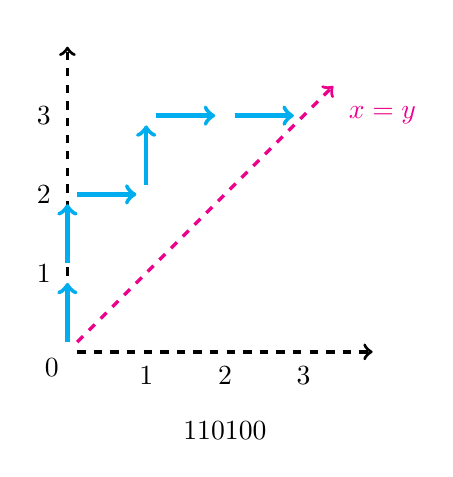
\begin{tikzpicture}[scale = 1]
            \node (a) at (0, 0) {};
            \node (b) at (0, 4) {};
            \node (c) at (4, 0) {};
            \node (d) at (3.5, 3.5) {};
            \node (e) at (4, 3) [color = magenta]
                {$x = y$}; 
            \draw [dashed, very thick, ->] (a) to (b);
            \draw [dashed, very thick, ->] (a) to (c);
            \draw [dashed, very thick, ->]
                [color = magenta] (a) to (d);

            \node (1)  at (0,0)   {};
            \node (2)  at (0,1)   {};
            \node (3)  at (0,2)   {};
            \node (4)  at (1,2)   {};
            \node (5)  at (1,3)   {};
            \node (6)  at (2,3)   {};
            \node (7)  at (3,3)   {};
            \draw [->, ultra thick, color = cyan]
                (1)  to (2);
            \draw [->, ultra thick, color = cyan] 
                (2)  to (3);
            \draw [->, ultra thick, color = cyan]
                (3)  to (4);
            \draw [->, ultra thick, color = cyan]
                (4)  to (5);
            \draw [->, ultra thick, color = cyan]
                (5)  to (6);
            \draw [->, ultra thick, color = cyan]
                (6)  to (7);

            \node at (-0.2, -0.2) {$0$};
            \node at (-0.3, 1)    {$1$};
            \node at (1, -0.3)    {$1$};
            \node at (-0.3, 2)    {$2$};
            \node at (2, -0.3)    {$2$};
            \node at (-0.3, 3)    {$3$};
            \node at (3, -0.3)    {$3$};
            \node at (2, -1)      {$110100$};
        \end{tikzpicture}
\end{expl}

\begin{expl}[$a > b$]
    ~
    \begin{itemize}
        \item $a = 9$
        \item $b = 7$
        \item Limites : $[1,\ 1 \frac{7}{9},\ 
            2 \frac{5}{9},\ 3 \frac{3}{9},\  
            4 \frac{1}{9},\ 4 \frac{8}{9},\ 
            5 \frac{6}{9},\ 6 \frac{4}{9},\ 
            7 \frac{2}{9},\ 8]$
        \item Limites entières : $[0,1,1,2,3,4,4,5,6,7,8]$
        \item Intervalles :
            \subitem $]0, 1]$ \hspace{5mm} $]1, 1]$
            \hspace{5mm} $]1, 2]$ \hspace{5mm} $]2, 3]$
            \hspace{5mm} $]3, 4]$ 
            \subitem $]4, 4]$ \hspace{5mm} $[4, 5]$
            \hspace{5mm} $]5, 6]$ \hspace{5mm} $]6, 7]$
            \hspace{5mm} $]7, 8]$
        \item Groupes d'enfants :
            \subitem $[1]$ \hspace{5mm} $\emptyset$ 
            \hspace{5mm} $[2]$ \hspace{5mm} $[3]$
            \hspace{5mm} $[4]$ \hspace{5mm} $\emptyset$
            \hspace{5mm} $[5]$ \hspace{5mm} $[6]$
            \hspace{5mm} $[7]$ \hspace{5mm} $[8]$
        \item $f = (4,2,2,1,4,5,7,4,1)$
        \item Etiquettes : $\{\{4,9\},\ \{2,3\},\ \emptyset,\ 
            \{1,5,8\}, \{6\},\ \emptyset,\ \{7\},\ 
            \emptyset\}$\\
    \end{itemize}
    \begin{center}
    \begin{tikzpicture}[scale=0.75]
        \node (1)  at (0,17)   {$\{4,9\}$};
        \node (2)  at (0,13)   {$\{2,3\}$};
        \node (4)  at (3,9)   {$\{1,5,8\}$};
        \node (5)  at (0,5)    {$\{6\}$};
        \node (7)  at (6,5)    {$\{7\}$};

        \node (a) at (-1.5,17)    {$1$};
        \node (b) at (-1.5,13)    {$2$};
        \node (c) at (-2,11)      {$3$};
        \node (d) at (1.5,9)      {$4$};
        \node (e) at (1.5,5)      {$5$};
        \node (f) at (-1,3)       {$6$};
        \node (g) at (4.5,5)      {$7$};
        \node (h) at (5,3)        {$8$};

        \node[right] (ac) at (1.5,17) {$2$ groupes d'enfants : $\emptyset$
         et $[2]$};
        \node[right] (bc) at (1.5,13) {$2$ groupes d'enfants : $[3]$
         et $[4]$};
        \node[right] (dc) at (4.5,9) {$3$ groupes d'enfants : $\emptyset$,
         $[5]$ et $[7]$};
        \node[left] (fc) at (-1.5,5) {$1$ groupe d'enfants : $[6]$};
        \node[right] (gc) at (7.5,5) {$1$ groupe d'enfants : $[8]$};

        \draw[ultra thick][color=brown!70!orange]
            (0,17)  circle (1);
        \draw[ultra thick][color=brown!70!orange]
            (0,13) circle (1);
        \draw[ultra thick][color=brown!70!orange]
            (3,9)  circle (1);
        \draw[ultra thick][color=brown!70!orange]
            (0,5)  circle (1);
        \draw[ultra thick][color=brown!70!orange]
            (6,5)  circle (1);

        \draw [->][ultra thick][color=brown!70!orange]
            (0,16) to (0,14.2);
        \draw [->][ultra thick][color=brown!70!orange]
            (0.6,12.25) to (2.7,10.2);
        \draw [->][ultra thick][color=brown!70!orange]
            (2.4,8.25) to (0.3,6.2);
        \draw [->][ultra thick][color=brown!70!orange]
            (3.6,8.25) to (5.7,6.2);

        \draw [-*][ultra thick][color=green!60!gray]
            (-0.6,12.2) to (-1.6,11);
        \draw [-*][ultra thick][color=green!60!gray]
            (0,4) to (0,3);
        \draw [-*][ultra thick][color=green!60!gray]
            (6,4) to (6,3);
    \end{tikzpicture}
\end{center}
\end{expl}

Dans les deux cas, la direction inverse de la \emph{bijection} est obtenue
-- comme pour le cas classique -- par un parcours préfixe.